\documentclass[12pt,titlepage]{article}
\usepackage[margin=1.25in]{geometry}
\usepackage{graphicx,amsmath,minted}

%% Variables definition
\newcommand{\vSubject}{Advanced Web Programming}
\newcommand{\vSubtitle}{Setup}
\newcommand{\vName}{Dicha Zelianivan Arkana}
\newcommand{\vNIM}{2241720002}
\newcommand{\vClass}{2i}
\newcommand{\vDepartment}{Information Technology}
\newcommand{\vStudyProgram}{D4 Informatics Engineering}

%% [START] Tikz related stuff
\usepackage{tikz}
\usetikzlibrary{svg.path,calc,shapes.geometric,shapes.misc}
\tikzstyle{terminator} = [rectangle, draw, text centered, rounded corners = 1em, minimum height=2em]
\tikzstyle{preparation} = [chamfered rectangle, chamfered rectangle sep=0.75em, draw, text centered, minimum height = 2em]
\tikzstyle{process} = [rectangle, draw, text centered, minimum height=2em]
\tikzstyle{decision} = [diamond, aspect=2, draw, text centered, minimum height=2em]
\tikzstyle{data}=[trapezium, draw, text centered, trapezium left angle=60, trapezium right angle=120, minimum height=2em]
\tikzstyle{connector} = [line width=0.25mm,->]
%% [END] Tikz related stuff

%% [START] Fancy header related stuff
\usepackage{fancyhdr}
\pagestyle{fancy}
\setlength{\headheight}{15pt} % compensate fancyhdr style
\fancyhead{}
\fancyfoot{}
\fancyfoot[L]{\thepage}
\fancyfoot[R]{\textit{\vSubject - \vSubtitle}}
\renewcommand{\footrulewidth}{0.4pt}% default is 0pt, overline for footer
%% [END] Fancy header related stuff

%% [START] Custom tabular command related stuff
\usepackage{tabularx}
\newcommand{\details}[2]{
    #1 & #2  \\
}
%% [END] Custom tabular command related stuff

%% [START] Figure related stuff
\newcommand{\image}[3][1]{
    \begin{figure}[h]
        \centering
        \includegraphics[#1]{#2}
        \caption{#3}
        \label{#3}
    \end{figure}
}
%% [END] Figure related stuff

\begin{document}
\begin{titlepage}
    \centering
    \vfill
    {\bfseries\LARGE
        \vSubject\\
        \vskip0.25cm
        \vSubtitle
    }
    \vfill
    
\includegraphics[width=6cm]{images/polinema-logo.png}
    \vfill
    {
        \textbf{Name}\\
        \vName\\
        \vskip0.5cm
        \textbf{NIM}\\
        \vNIM\\
        \vskip0.5cm
        \textbf{Class}\\
        \vClass\\
        \vskip0.5cm
        \textbf{Department}\\
        \vDepartment\\
        \vskip0.5cm
        \textbf{Study Program}\\
        \vStudyProgram
    }
\end{titlepage}

\section{Web Server}

I'm using Linux, so Laragon is not available for me. I've been using Laravel Sail for my development
environment when using Laravel this past 2 years or so. It's Docker-based so it can run anywhere
and portable. Moreover, it's very easy to use and doesn't require a lot of configuration.

It uses the builtin PHP web server since it's good enough for development.
Although it is recommended to use NGINX instead for production.

I installed \texttt{sail} using this command, which will basically scaffold the project while setting up
the required services such as the database.

\begin{minted}[fontsize=\small,autogobble]{java}
    curl -s "https://laravel.build/my-application-name?with=mysql" | bash
\end{minted}

Here's an example output, it should start installing the required 
dependencies and pulling docker images. It will take a while
since it's going to download a lot of things.

\begin{center}
    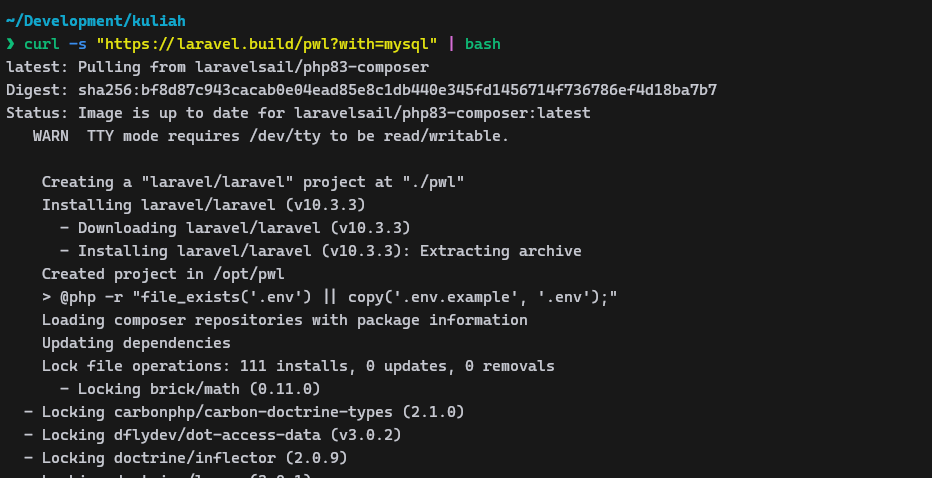
\includegraphics[width=.8\textwidth]{./images/sail-installation.png}
\end{center}

The project can still be used with or without Laravel Sail. It's just an option
if you don't want to install PHP, Composer, and MySQL on your local machine.

\pagebreak

\section{Text Editor / IDE}
I use Intellij IDEA Ultimate for my main IDE. I already use it for other languages
so why bother installing another IDE which is basically just a stripped down
version of it. In terms of developer experience, they're the same. Probably some
small difference in project template but that's it. Not using it anyway.

\vspace*{5mm}


\includegraphics[width=.4\textwidth]{./images/jetbrains-toolbox.png}

\section{Git}

I'm using Git installed from the official Fedora repository,
which at the time of writing this, is version 2.43.0 as shown below.

\vspace*{5mm}


\includegraphics[width=.6\textwidth]{./images/git.png}

\pagebreak

\section{Committing to Github}
I'm using Git from the CLI to commit to Github. I've made the repository previously
on Github. I'm using the following commands to commit to Github.

\vspace*{5mm}

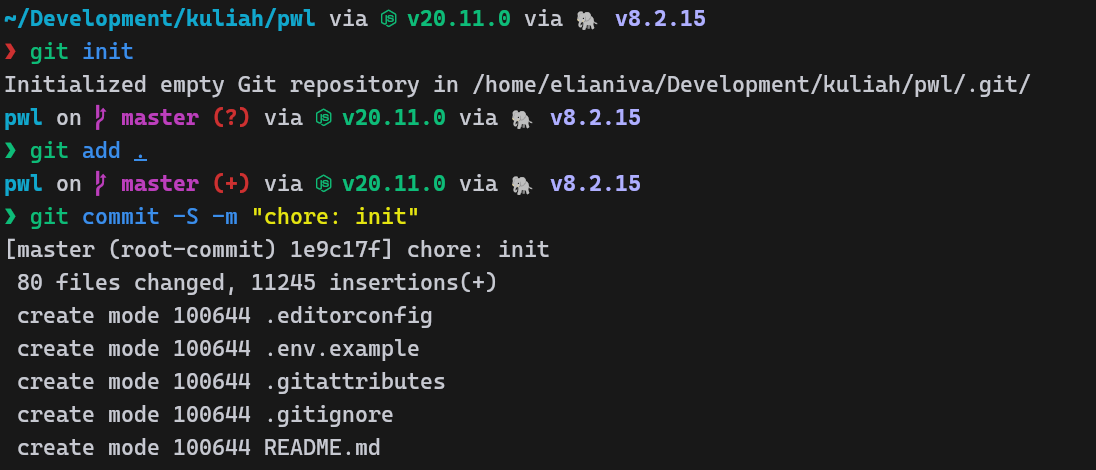
\includegraphics[width=.6\textwidth]{./images/git-1.png}

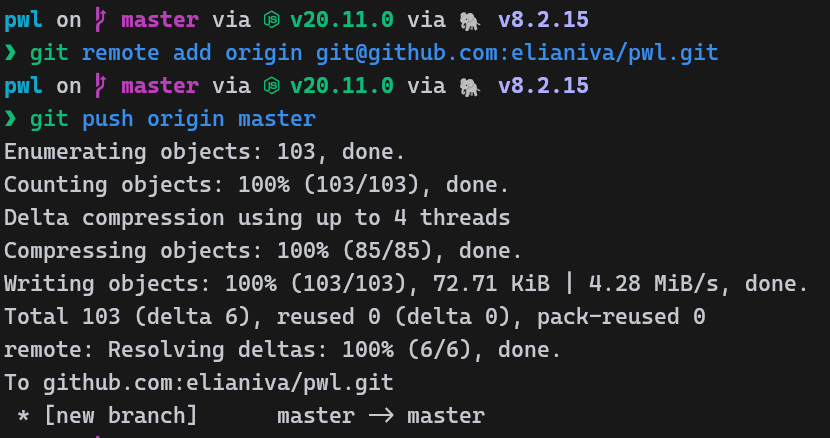
\includegraphics[width=.6\textwidth]{./images/git-2.png}

It basically initialised the repository, added the files to the staging area,
creating a signed commit with a commit message, adding a remote repository,
and then pushing it to Github.

\end{document}

